\documentclass{beamer}
\usepackage{xcolor}  
\usepackage{tikz}
\usepackage{geometry}
\usepackage{graphicx}
\usepackage{amsmath}
\usepackage{amssymb}
\usepackage{enumitem}
\usepackage{xcolor}
\usepackage{listings}
\usepackage{threeparttable}
\usepackage{multirow}
\usepackage{longtable}
\usetikzlibrary{arrows,shapes,chains}  
\setbeamertemplate{caption}[numbered]
\setbeamertemplate{bibliography item}[text]

\mode<presentation> {
\usepackage[UTF8]{ctex}
\usepackage{amsmath}
\usetheme{Madrid}
\usepackage{graphicx} % Allows including images
\usepackage{booktabs} % Allows the use of \toprule, 
}

%----------------------------------------------------------------------------------------
%	TITLE PAGE
%----------------------------------------------------------------------------------------
\title[] %optional
{NumPDE Project3 分享}

\author[]
{强基数学2001班-樊睿}
\date[2023年6月6日] % (optional)
{2023年6月6日}

\AtBeginSection[]
{
  \begin{frame}
    \frametitle{Table of Contents}
    \tableofcontents[currentsection]
  \end{frame}
}

\begin{document}

\frame{\titlepage}

\begin{frame}{设计文档}	
	\centering  
	\begin{figure}  
		\scriptsize  
		\tikzstyle{format}=[rectangle,draw,thin,fill=white]  
		\tikzstyle{test}=[diamond,aspect=2,draw,thin]
		\tikzstyle{point}=[coordinate,on grid,]
		\begin{tikzpicture}
		\node[format] (p1){IVPSolver};
		\node[point,below of=p1,node distance=7mm] (o3){};
		\node[point,left of=o3,node distance=35mm] (o2){};
		\node[point,right of=o3,node distance=35mm] (o4){};
		\node[format,below of=o3,node distance=8mm] (p3){RK};
		\node[format,below of=o2,node distance=8mm] (p2){LMM};
		\node[format,below of=o4,node distance=8mm] (p4){Emb-RK};
		
		\node[point,below of=p3, node distance=7mm] (q3){};
		\node[point,left of=q3, node distance=7mm] (o5){};
		\node[point,right of=q3, node distance=7mm] (o6){};
		\node[format,below of=o5,node distance=8mm] (p5){ERK};
		\node[format,below of=o6,node distance=8mm] (p6){IRK};
		
		\node[point,below of=p2,node distance=7mm] (o8){};
		\node[point,left of=o8,node distance=24mm] (o7){};
		\node[point,right of=o8,node distance=18mm] (o9){};
		\node[format,below of=o8,node distance=8mm] (p8){Adam-Moulton};
		\node[format,below of=o7,node distance=8mm] (p7){Adam-Bashforth};
		\node[format,below of=o9,node distance=8mm] (p9){BDF};
		
		\node[point,below of=p4, node distance=7mm] (q4){};
		\node[point,left of=q4, node distance=12mm] (o10){};
		\node[point,right of=q4, node distance=14mm] (o11){};
		\node[format,below of=o10,node distance=8mm] (p10){Fehlberg};
		\node[format,below of=o11,node distance=8mm] (p11){Dormand-Prince};

		\node[point,below of=p5, node distance=7mm] (q5){};
		\node[point,left of=q5, node distance=15mm] (o12){};
		\node[format,below of=o12,node distance=8mm] (p12){Classical-4th-RK};

		\node[point,below of=p6, node distance=7mm] (q6){};
		\node[point,left of=q6, node distance=8mm] (o13){};
		\node[point,right of=q6, node distance=10mm] (o14){};
		\node[format,below of=o13,node distance=8mm] (p13){ESDIRK};
		\node[format,below of=o14,node distance=8mm] (p14){Gauss-Legendre};

		\node[format,right of=p1,node distance=45mm] (p15){Matrix};
		\node[format,below of=p15,node distance=5mm] (p16){Function};

		\draw[-](p1)--(o3);
		\draw[-](o3)--(o2);
		\draw[-](o3)--(o4);
		\draw[-](o2)--(p2);
		\draw[-](o3)--(p3);
		\draw[-](o4)--(p4);
		\draw[-](p3)--(q3);
		\draw[-](q3)--(o5);
		\draw[-](q3)--(o6);
		\draw[-](o5)--(p5);
		\draw[-](o6)--(p6);
		\draw[-](p2)--(o8);
		\draw[-](o8)--(o7);
		\draw[-](o8)--(o9);
		\draw[-](o7)--(p7);
		\draw[-](o8)--(p8);
		\draw[-](o9)--(p9);
		\draw[-](p4)--(q4);
		\draw[-](q4)--(o10);
		\draw[-](q4)--(o11);
		\draw[-](o10)--(p10);
		\draw[-](o11)--(p11);
		\draw[-](p5)--(q5);
		\draw[-](q5)--(o12);
		\draw[-](o12)--(p12);
		\draw[-](p6)--(q6);
		\draw[-](q6)--(o13);
		\draw[-](q6)--(o14);
		\draw[-](o13)--(p13);
		\draw[-](o14)--(p14);

		\end{tikzpicture}
	\end{figure}
\end{frame}


\begin{frame}{多步法的初值}

当 $s=1$(即一步法)时,直接令 $U^0=u_0$ 并迭代 $n$ 步即可。

但当 $s>1$ 时,因为我们至少要 $s$ 个初值 $U^0,U^1,\dots,U^{s-1}$,而后 $s-1$ 个初值并非已知,所以我们需要用其他方法计算出这些初值。

最简单的做法是直接用对应的一步法计算。但一步法的误差是 $O(k)$ 的,而我们知道常微分方程组的误差是累乘的,因此这会导致最终用高阶多步法解出的答案和用一步法解出的答案差不多。这样高阶多步法就失去意义了。

另一种做法是用高阶单步法(例如四阶RK方法、三阶Gauss-Legerand方法等)计算前 $s-1$ 个初值,这样可以保证高阶多步法的精度。但这样在使用多步法的同时还要使用其他单步法,某种意义上也使多步法失去了它的精髓。

\end{frame}

\begin{frame}{本项目的解决方案}
本项目中采取的做法是使用 $s-1$ 阶单步法计算前 $s-1$ 个初值,但缩短时间步长。设原 $s$ 阶多步法步长为 $k$,则令 $s-1$ 阶单步法步长为 $k^{\frac s{s-1}}$。

当然,如果 $s-1\geq 2$,这 $s-1$ 个初值也不能直接计算。因此要继续递归,直到 $s=1$ 为止。

然而,这样又引出了下一个问题。例如我们取 $T=1,s=4,k=10^{-4}$,则递归到 $s=1$ 时,我们需要以 $10^{-16}$ 的步长计算 $t=10^{-8}$ 处的值。这样需要迭代 $10^8$ 步!这远远超过了原本所需迭代的次数 $10^4$。

不难证明只有 $s=2$ 时下一步递归会出现这种情况。考虑倍增优化,设 $s=2$ 时步长为 $k$,我们先用单步法计算 $0,k^2$ 处的值,然后用 $s=2$ 的多步法以 $0,k^2$ 处的初值计算 $2k^2$ 处的值,再用 $0,2k^2$ 处的初值计算 $4k^2$ 处的值,直到计算出 $k$ 处的值为止。

这样第一步的误差是 $O(k^2)$,而后面每一步的误差都至多 $O(k^2)$。步数是 $O(\log k)$。这样就避免了严重耗时的问题。

\end{frame}

\begin{frame}{测试结果与分析}

	\begin{table}\centering
		\resizebox{0.75\columnwidth}{!}{
		\begin{tabular}{|c|c|c|c|c|c|c|c|c|c|c|c|c|}
		\hline
		\multirow{2}{*}{迭代步数} & \multicolumn{3}{c|}{$s=1$} & \multicolumn{3}{c|}{$s=2$} & \multicolumn{3}{c|}{$s=3$} & \multicolumn{3}{c|}{$s=4$} \\ \cline{2-13}
		& 误差 & 时间 & 收敛阶 & 误差 & 时间 & 收敛阶 & 误差 & 时间 & 收敛阶 & 误差 & 时间 & 收敛阶\\ \cline{1-13}
		$5\times 10^5$ & 1.79e+00 & 647  & - & 8.38e-01 & 1278 & - & 3.96e-03 & 1936 & - & 4.57e-04 & 2537 & - \\ \cline{1-13}
		$1\times 10^6$ & 1.71e+00 & 1426 & 0.07 & 2.00e-01 & 2597 & 2.07 & 5.17e-04 & 3862 & 2.93 & 2.89e-05 & 4925 & 3.98\\ \cline{1-13}
		$2\times 10^6$ & 1.59e+00 & 2837 & 0.10 & 4.84e-02 & 5126 & 2.05 & 6.60e-05 & 7730 & 2.97 & 1.82e-06 & 9703 & 4.16\\ \cline{1-13}
		\end{tabular}}
		\caption{Adam-Bashforth方法的误差和效率}
	\end{table}

	\begin{table}\centering
		\resizebox{0.75\columnwidth}{!}{
		\begin{tabular}{|c|c|c|c|c|c|c|c|c|c|c|c|c|}
		\hline
		\multirow{2}{*}{迭代步数} & \multicolumn{3}{c|}{$s=1$} & \multicolumn{3}{c|}{$s=2$} & \multicolumn{3}{c|}{$s=3$} & \multicolumn{3}{c|}{$s=4$} \\ \cline{2-13}
		& 误差 & 时间 & 收敛阶 & 误差 & 时间 & 收敛阶 & 误差 & 时间 & 收敛阶 & 误差 & 时间 & 收敛阶\\ \cline{1-13}
		$5\times 10^5$ & 1.46e-01 & 5848 & - & 3.11e+00 & 7746 & - & 1.83e-01 & 9526 & - & 4.44e-03 & 11239 & - \\ \cline{1-13}
		$1\times 10^6$ & 3.79e-02 & 10757 & 1.95 & 3.08e+00 & 13850 & - & 5.21e-02 & 18293 & 1.81 & 9.86e-04 & 22053 & 2.17 \\ \cline{1-13}
		$2\times 10^6$ & 9.55e-03 & 19692 & 1.99 & 3.07e+00 & 27927 & - & 1.53e-02 & 35342 & 1.77 & 2.40e-04 & 45365 & 2.03 \\ \cline{1-13}
		\end{tabular}}
		\caption{Adam-Moulton方法的误差和效率}
	\end{table}
	
	\begin{table}\centering
		\resizebox{0.75\columnwidth}{!}{
		\begin{tabular}{|c|c|c|c|c|c|c|c|c|c|c|c|c|}
		\hline
		\multirow{2}{*}{迭代步数} & \multicolumn{3}{c|}{$s=1$} & \multicolumn{3}{c|}{$s=2$} & \multicolumn{3}{c|}{$s=3$} & \multicolumn{3}{c|}{$s=4$} \\ \cline{2-13}
		& 误差 & 时间 & 收敛阶 & 误差 & 时间 & 收敛阶 & 误差 & 时间 & 收敛阶 & 误差 & 时间 & 收敛阶\\ \cline{1-13}
		$5\times 10^5$ & 2.10e+00 & 5981 & - & 4.96e-01 & 5812 & - & 2.53e-03 & 6748 & - & 2.62e-04 & 6958 & - \\ \cline{1-13}
		$1\times 10^6$ & 2.12e+00 & 8040 & - & 1.46e-01 & 9457 & 1.76 & 3.36e-04 & 11283 & 2.91 & 1.73e-05 & 12726 & 3.92 \\ \cline{1-13}
		$2\times 10^6$ & 2.33e+00 & 14604 & - & 3.78e-02 & 17695 & 1.94 & 4.09e-05 & 20293 & 3.03 & 2.40e-06 & 23632 & 2.85\\ \cline{1-13}
		\end{tabular}}
		\caption{BDF方法的误差和效率}
	\end{table}
	
\end{frame}

\begin{frame}{测试结果与分析}
	下面分别给出三种方法的最高阶方法对第一组初值和周期的作图。两个周期。

	\begin{figure}[htbp]
		\begin{minipage}{4cm}
			\centering
			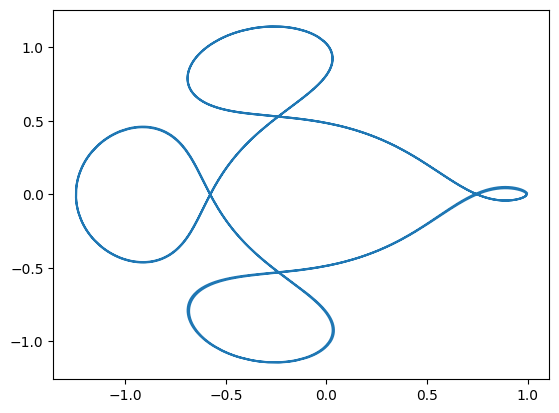
\includegraphics[width = 3cm, height = 2cm]{11.png}
			\caption{Adam-Bashforth, $s=4,n=500000$}
			\label{11}
		\end{minipage}
		\begin{minipage}{4cm}
			\centering
			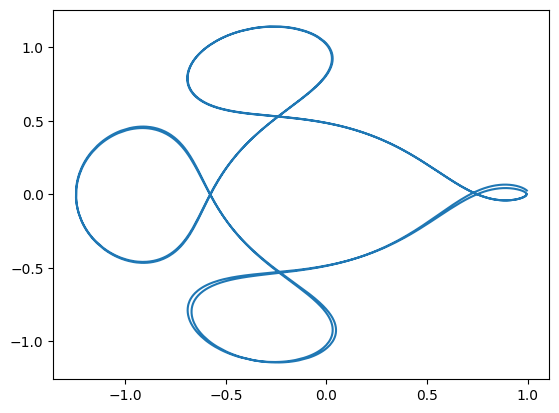
\includegraphics[width = 3cm, height = 2cm]{12.png}
			\caption{Adam-Moulton, $s=4,n=500000$}
			\label{12}
		\end{minipage}
		\begin{minipage}{4cm}
			\centering
			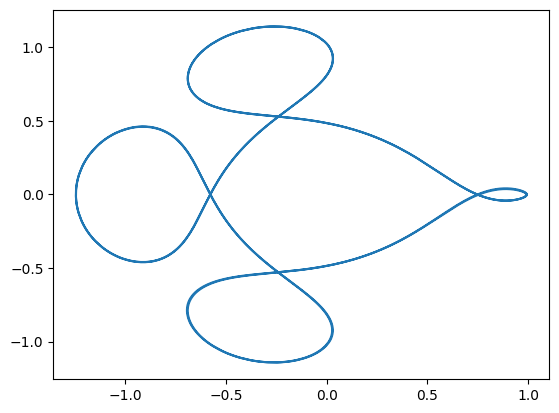
\includegraphics[width = 3cm, height = 2cm]{13.png}
			\caption{BDF, $s=4,n=500000$}
			\label{13}
		\end{minipage}
	\end{figure}	
\end{frame}

\begin{frame}{存在的不足}
	多步法在 $s=1$ 时,步长可能会达到 $10^{-20}$ 级别,超出机器精度,导致无法正常迭代。这可能也是后两种多步法无法收敛的原因。

	若想让它们达到理论精度,可能只能用超高精度的数据类型了。
\end{frame}

\begin{frame}
\Huge{\centerline{谢谢!}}
\end{frame}
\end{document}